%==========================================================================

\begin{frame}[fragile]

  {\Huge Backend Updates}

  \vspace{10pt}

\end{frame}


%==========================================================================

% Examples

% note: always keep the [fragile] for your frames!

\begin{frame}[fragile]{CUDA, SYCL and Serial}
  \begin{itemize}
      \item CUDA: Improved performance for \texttt{Kokkos::parallel\_reduce} on H100 and newer by removing limitations on the runtime thread configuration
      \item SYCL: Improved sorting performance for non-contiguous views
      \item Serial: Reduce fences overhead when using \texttt{Kokkos\_ENABLE\_ATOMICS\_BYPASS}
  \end{itemize}
\end{frame}

%==========================================================================
\begin{frame}[fragile]{Performance of \texttt{parallel\_reduce}}

  \begin{center}
    \begin{minipage}{.45\textwidth}
    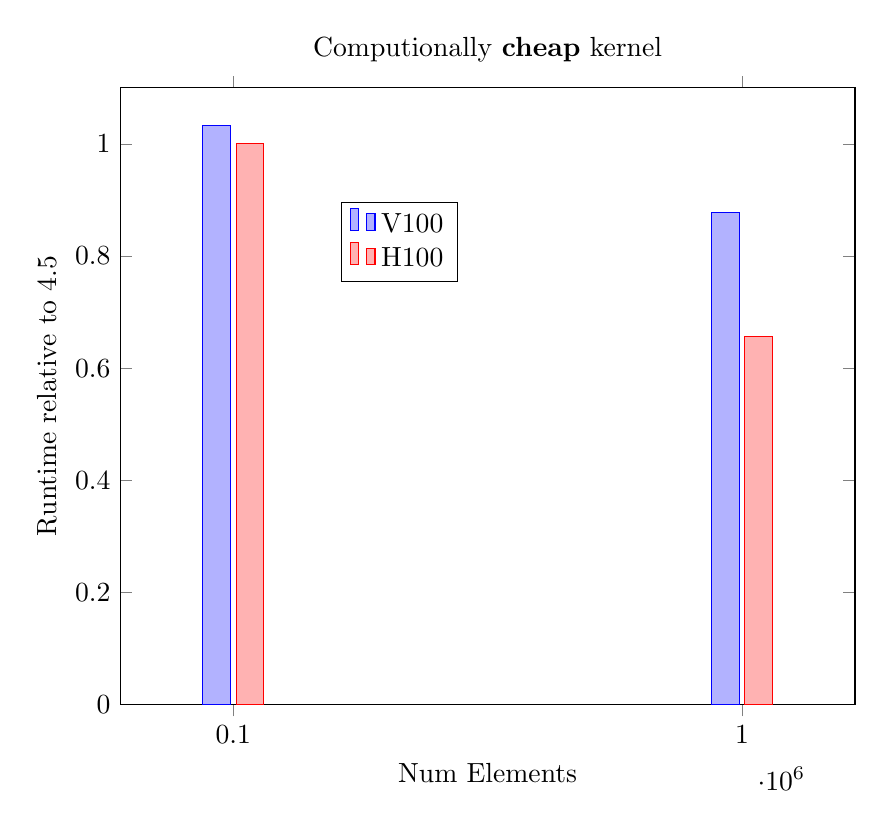
\begin{tikzpicture}
	\begin{axis}[
      title={Computionally \textbf{cheap} kernel},
    ymin=0,
    ymax=1.1,
    xmin=-100000,
    xmax=1200000,
    ybar,
    xtick={100000,1000000},
    width=0.9\textwidth,
    legend style={at={(0.3,0.75)},anchor=west},
		xlabel=Num Elements,
    ylabel=Runtime relative to 4.5]
  \addplot coordinates {(100000,1.033333333) (1000000,0.876923077)};
  \addplot coordinates {(100000,1.0) (1000000,0.6559139)};
  \legend{V100,H100}
	\end{axis}
\end{tikzpicture}
\end{minipage}
\begin{minipage}{.45\textwidth}
    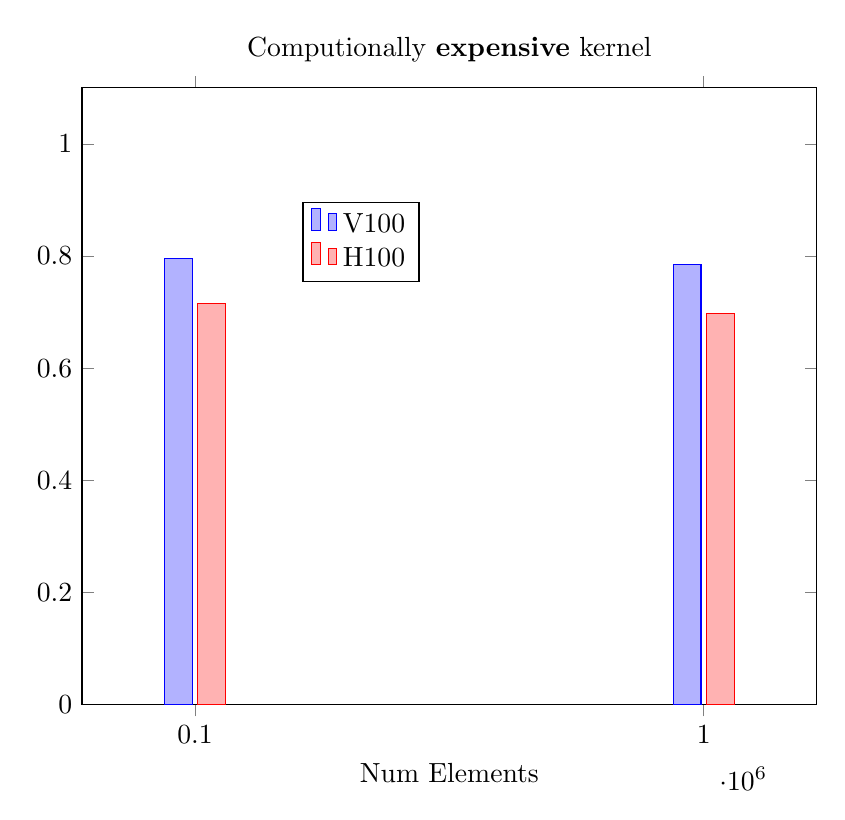
\begin{tikzpicture}
	\begin{axis}[
      title={Computionally \textbf{expensive} kernel},
    ymin=0,
    ymax=1.1,
    xmin=-100000,
    xmax=1200000,
    ybar,
    xtick={100000,1000000},
    width=0.9\textwidth,
    legend style={at={(0.3,0.75)},anchor=west},
		xlabel=Num Elements,
    % ylabel=Speedup relative to 4.5,
  ]
  \addplot coordinates {(100000,0.7956778) (1000000,0.785453609)};
  \addplot coordinates {(100000,0.7149638336) (1000000,0.6977690684)};
  \legend{V100,H100}
	\end{axis}
\end{tikzpicture}
\end{minipage}
  \end{center}

\end{frame}
%==========================================================================

\begin{frame}[fragile]{HIP}
  \begin{itemize}
      \item Change block size deduction to prefer smaller blocks/teams if possible
      \item Allocate memory with stream ordered semantics (\emph{i.e.}\ use \texttt{hipMallocAsync})
      \item Fix a segfault when a virtual function called inside a kernel requires too many registers
  \end{itemize}
\end{frame}

%==========================================================================


%==========================================================================

